\documentclass[conference]{IEEEtran}

% *** CITATION PACKAGES ***
%
\usepackage{cite}
% cite.sty was written by Donald Arseneau
% V1.6 and later of IEEEtran pre-defines the format of the cite.sty package
% \cite{} output to follow that of IEEE. Loading the cite package will
% result in citation numbers being automatically sorted and properly
% "compressed/ranged". e.g., [1], [9], [2], [7], [5], [6] without using
% cite.sty will become [1], [2], [5]--[7], [9] using cite.sty. cite.sty's
% \cite will automatically add leading space, if needed. Use cite.sty's
% noadjust option (cite.sty V3.8 and later) if you want to turn this off.
% cite.sty is already installed on most LaTeX systems. Be sure and use
% version 4.0 (2003-05-27) and later if using hyperref.sty. cite.sty does
% not currently provide for hyperlinked citations.
% The latest version can be obtained at:
% http://www.ctan.org/tex-archive/macros/latex/contrib/cite/
% The documentation is contained in the cite.sty file itself.

\usepackage[pdftex]{graphicx}
\graphicspath{{rec/}}
\DeclareGraphicsExtensions{.pdf,.jpeg,.png}

\usepackage[cmex10]{amsmath}
\interdisplaylinepenalty=2500

\usepackage{algorithmic}
\usepackage{array}
\usepackage{mdwmath}
\usepackage{mdwtab}
\usepackage{eqparbox}

\usepackage[tight,footnotesize]{subfigure}

%\usepackage{fixltx2e} % This seams to cause issues with two-column figures.
\usepackage{stfloats}

\usepackage{url}

% correct bad hyphenation here
\hyphenation{op-tical net-works semi-conduc-tor}

\begin{document}
%
% paper title
% can use linebreaks \\ within to get better formatting as desired
\title{CPPN Based Evolution of Bitmap Facial Distortion}


% author names and affiliations
% use a multiple column layout for up to three different
% affiliations
\author{\IEEEauthorblockN{James Schneider}
\IEEEauthorblockA{School of Electrical Engineering and \\Computer Science\\
University of Central Florida\\
Orlando, FL 32816\\
Email: jschneider@knights.ucf.edu}
\and
\IEEEauthorblockN{Anthony Wertz}
\IEEEauthorblockA{School of Electrical Engineering and \\Computer Science\\
University of Central Florida\\
Orlando, FL 32816\\
Email: awertz@knights.ucf.edu}}

% make the title area
\maketitle

\begin{abstract}
Hello, my name is Picasso

\end{abstract}

% For peerreview papers, this IEEEtran command inserts a page break and
% creates the second title. It will be ignored for other modes.
\IEEEpeerreviewmaketitle

\section{Introduction}
The diversity that appears on planet Earth is broad but reuse is a common trait among all animals. Each face is 
complex in its own right, but what is the ultimate limit in possible facial configurations? Each facial structure
is evolved to attract mates and/or optimize placement of sensors to increase survivability. The possible configurations
of faces though is limited by multiple factors such as weight, surface area, etc. these factors place an upper limit
on the possible faces that can be seen on the planet Earth. These optimization factors combined with the non-random 
starting point of currently available facial structures converts an immeasurable problem to one of surprisingly low
dimensionality \cite{sirovich1987low}. This paper will focus on human and human-like faces for its distortions.

Human like faces are interesting in that they demonstrate the property of repeatability with variation \cite{stanley2007compositional}.
Most animal faces exhibit these same qualities as well, though seeing a warped animal face may not seem as interesting to
a human observer compared with a distortion of a human face since the incongruities of distorted faces in members of his or her own
species seem a bit more disturbing. This process due potentially to facial recognition circuits buried deep within the human brain that have evolved
for quick unsupervised feature detection and identification in conjunction with other circuitry designed to recognize specifically members of
the human race. This understandability of the interestingness of evolved faces directly ties to the ability to quickly verify
results obtained by the algorithmic process and is a cornerstone to this paper's research.

The overall goal of this paper is to produce new plausible facial structures and explore how these facial structures evolve. Though,
as mentioned earlier, the dimensionality for human faces is bounded, this bound is unexplored. Taking this into consideration
this paper will utilize a evolutionary process to search for new and novel faces. There are multiple search algorithms
in practice but most of them require some form of objective function and it is currently unknown how to objectify interesting faces.
Taking this into account this paper will utilize a user guided search where the individual determines what is interesting. This, though,
is not enough as the user may not know what is interesting until it is presented. The algorithm could be a random search but due to the
size of the search space it may require an unrealistically long duration before interesting results are uncovered. 

To solve these issues the algorithm used is NeuroEvolution and Augmenting Topologies \cite{stanley2002evolving} hereby referred to as NEAT.
NEAT allows for directed evolution of neural networks towards a goal using the concepts of speciation (evolving new species), historical markings,
and directed complexification. The NEAT process is utilized in conjunction with Compositional Pattern Producing Networks \cite{stanley2007compositional}
(CPPNs) and interactive evolution in order to evolve distortions more desirable to the human operator. This paper will seek to provide evidence that not
only can interesting images be found by humans but that these can be found with great efficiency and that, in the process of exploration, a
deeper process starts to unveil itself.

This paper will provide evidence that evolution of images needs not only a directed search but also an understanding of the domain
in order to correctly capture interesting facial structures. Exploration of the process and results of the evolution will take place
in this paper including examination of the interesting results gleaned. These results hint at some deeper understanding of not only what
humans find interesting but how human interaction changes the exploration and exploitation paradigm. This paper along with these
theoretical underpinnings explores an evolutionary architecture that produces more varied results and allows for faster exploitation
of those figures and features found in the exploration process.

Remove \cite{*} % Remove when we cite something.

\section{Background}
Neural Networks first appeared in literature as early as the 1960's, but until NEAT was introduced a user had to manually 
estimate the number of nodes needed to solve the proper and how these nodes were connected. In addition the network required
retraining every time new data was presented and failed to properly react to a changing objective function. These issues were
solved with the introduction of NEAT in 2002 \cite{stanley2002evolving}. NEAT evolves not only the weights of a network but
the placement of linkages and nodes inside of the network. This process is governed by a memorization genetic algorithm that 
seeks to optimize a user's fitness function. The major advantage of this system is the protection of innovation via speciation.
Speciation allows novel structures to survive long enough to eventually find a more optimal solution to the user's problem. 
This is important to the facial deformation problem as novel facial structures would be lost in any algorithm that vigoursly
explores the search space. Introducing the concept of speciation along with fitness sharing smooths out search space and 
allows semi-guided search to take place. The biggest issue with NEAT is that it still requires some user input in the form
of an objective. This domain input is needed in order for NEAT to decide if a structure is more correct than another, but 
this function describing images is currently not known. 

\begin{figure}
 \centering
 \label{fig:paper:CPNN}
 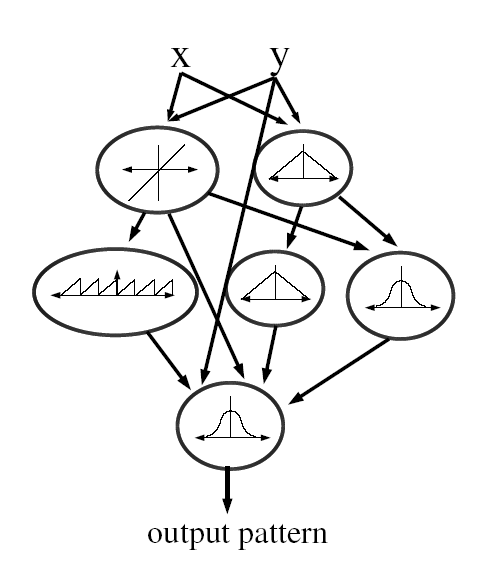
\includegraphics[height=1.5in,width=1.5in]{../../rec/paper/CPNN.png}
 \caption{CPNN Graph Abstraction} A graph abstraction of a compositional pattern producing neural network. The CPNN abstraction
 can be applied to a neural network type structure as the graph depicts \cite{stanley2002evolving}
\end{figure}

Due to the limitations of the NEAT process a second abstraction must be introduced in order to properly solve the facial 
deformation problem. CPNNs or Compositional Pattern Producing Networks are indirect encoded developmental networks that 
describe in a minimal set how something is created \cite{stanley2007compositional}. CPNNs eliminate two limitations the first
being a uniform activation function, and the second is sampling among a continuum rather than discrete points. Because CPNNs 
describe how a function evolves rather than how to evaluate a function CPNNs represent a different structure then that of 
artificial neural networks but one that can utilize the same structure of the networks \ref{fig:paper:CPNN}. The combination
of NEAT with the CPNN abstraction allows for greater ability to come up with a generational model for how a function develops
\cite{stanley2007compositional}.This process also allows for simplification of the fitness sharing metric involved in speciation
of the neural networks.In-lieu of a domain restricted optimization function the distance between the two networks can be used
to properly speciate the evolved networks \cite{stanley2007compositional}. Another fortuitous advantage of the algorithm is due
to the domain of images, as most images change in resolution and density more input neurons are not required as would be under
traditional neural network architectures. The CPNN ignores the resolution of the image and can generalize how the image is produced
thus saving valuable computational time.In addition, the process of including symmetrical activation functions with a generative process 
allows exclusion of large amounts of the search space allowing more efficient search for interesting artifacts. To this end the CPNN/NEAT
architecture allows interesting facial deformations to be discovered by the user in a timely and rigorous manner.

\begin{figure*}
 \centering
 \label{fig:paper:picbreed}
 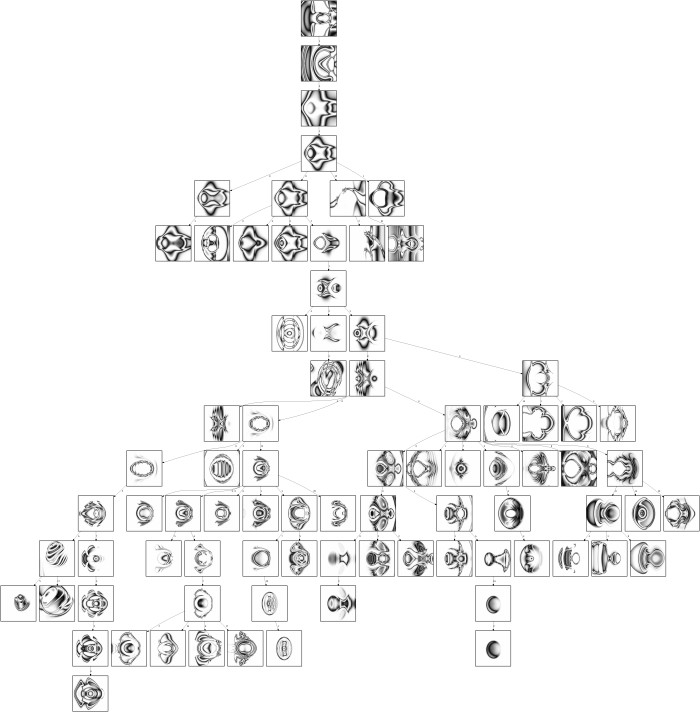
\includegraphics[height = 4in, width = 5in]{../../rec/paper/picbreed.jpg}
 \caption{PicBreeder} A graph abstraction of a compositional pattern producing neural network. The CPNN abstraction
 can be applied to a neural network type structure as the graph depicts \cite{stnaleypicbreed}
\end{figure*}

There still exists a issue to implementation of the algorithm and that is the objective function.Interestingness of a Human face is 
difficult to express in mathematical terms. Due to this limitation evolving interesting deformations with CPNN/NEAT is impossible.
There exists another abstraction that of Interactive Evolutionary Computation or IEC, IEC supplements a mathematical objective function
for one driven by a Human operator.Instead of performing a straight optimization route on images, Humans perform a meta-heuristic like search of the novel
spaces which encodes the optimal function this performs a search for interesting or novel entires \cite{lehman2010efficiently} \cite{li2009innovative}.  The CPNN/NEAT architecture has already been applied 
successfully to this domain with the inclusion of IEC \cite{secretan2008picbreeder}. PicBreeder allows for anyone with an Internet connection to evolve images from simple functions
into genetic art. The users of the site effectively perform a modified Gibbs sampling algorithm on the search space of interesting images.
This gives the PicBreeder program insight into the higher dimensional fitness function will still allowing CPNN/NEAT to evolve the underlaying
image representation. PicBreeder becomes a lesson in how to efficiently search through possible images, and its process becomes a cornerstone
of the facial deformation discovery process.

\section{Approach}
The CPNN/NEAT architecture is at the forefront of the facial deformation discovery process. The architecture takes 
advantage of developed software suites most notably HyperNEAT C++ \cite{jasongauci}. HyperNEAT C++ is a complete
version of NEAT, CPNN/NEAT and HyperNEAT that was suited to prove the validity of the HyperNEAT platform. 
Extensions to this original program had to be made in order to tailor it to the field of facial deformations. 
HyperNEAT C++ was extended with the Python programming language in order to create easier accessibility to the
underlying algorithmic process. The architecture presented in this paper is simple and allows for quick 
evaluation of image novelty by the user. The simple architecture \ref{fig:paper:architecture} allows for recursive 
processing of information in order to process not only static images but videos and allows expansion to
include more complex deformations including non Human faces.


\begin{figure*}
   \centering
    \subfigure[]{
        \centering
        \label{fig:paper:architecture}
        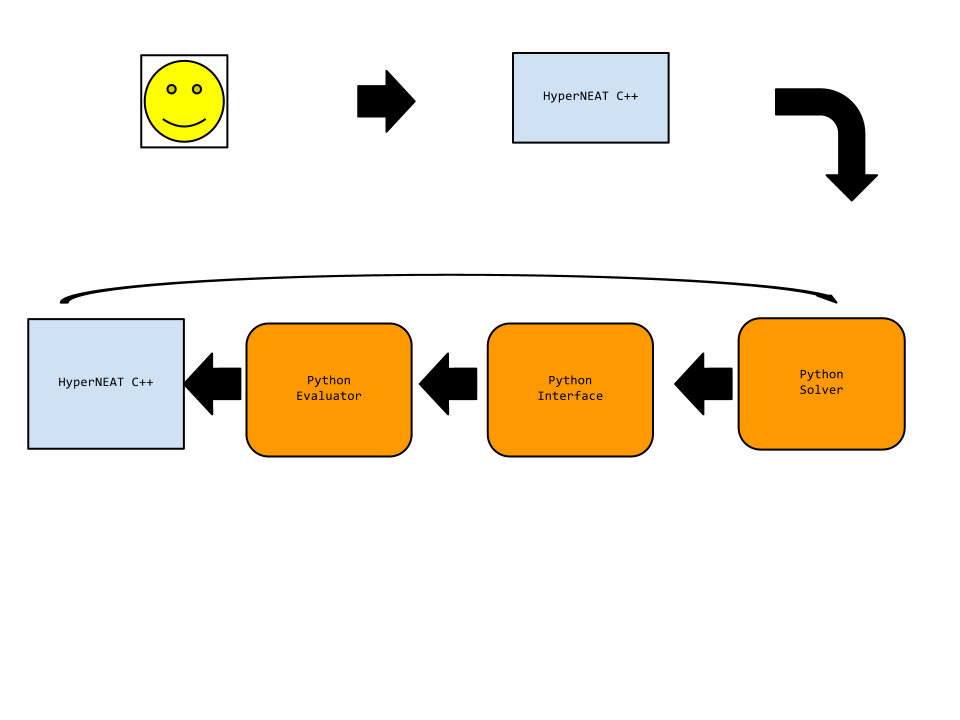
\includegraphics[height = 4in, width = 3in]{../../rec/paper/Face Deformations Architecture.png}
    }
    \subfigure[]{
       \label{fig:paper:interface}
        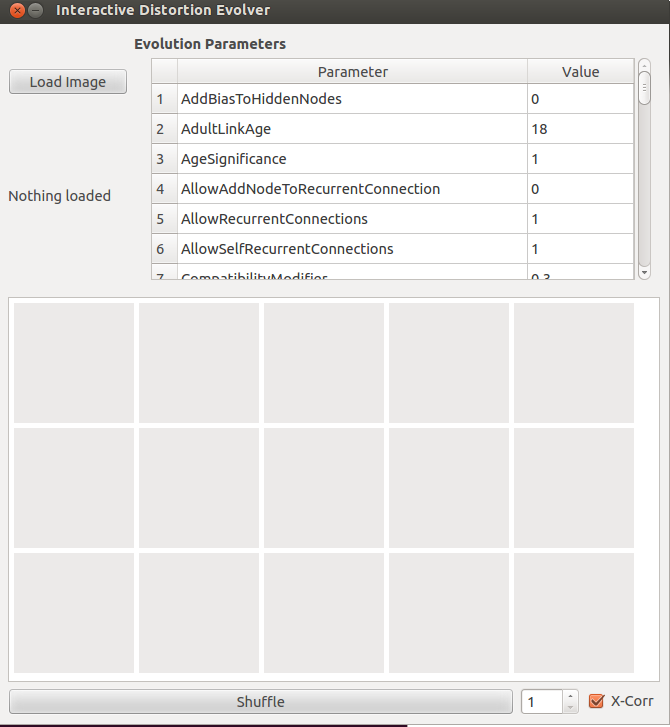
\includegraphics[height = 4in, width = 5in]{../../rec/paper/interface.png}
    }
    \caption{Facial deformations architecture and user interface for interactive evolution.}
\end{figure*}



The major issues with the architecture became obvious when running, the most glaring issue was that of user fatigue.
Cited in many major publications user fatigue is the anomaly that occurs when users are presented with a long search process
\cite{secretan2008picbreeder} \cite{li2009innovative}. Due to the constructive nature of genetic art in that each part or symmetry
is discovered in an orderly process and innovative structures are seldom seen by the user. Users frequently expect the innovative
images to be produced immediately, but this is inhibited by the expansive search space and no knowledge of what constitutes an 
mathematically interesting image. This problem is further exacerbated by the presence of noise in the genotype to phenotype 
representation. This noise takes the form of large changes to the underlying neural network structure producing relatively small
changes in the images. These small changes take the form of rotational and translational image transformations and represent the
phenotype of the large change in the genotype. It was discovered that these jumps occur more at lower complexity levels than at
larger levels and occur with a relative frequency. The combination of user fatigue, nonlinear mapping, and low complexity leads to
uninteresting images being produced by the algorithmic process. It is theorized that these issues would be solved given more users
with programs such as PicBreeder, as the process can be parallelized and utilize user histories to solve not only the fatigue issue
but also the complexity issues \cite{secretan2008picbreeder}.

Unable to acquire more users these issues had to be addressed in order for new novel structures to be discovered by the algorithmic
process. Using the insight that the novel structures represent something that has not been discovered before a novelty like search
algorithm can be implemented \cite{lehman2010efficiently}. The biggest hurdle is to discover a function of novelty of an image, this
was discovered by accident through observation. Using a image histogram a simple entropy calculation can be performed. This histogram
is then averaged over the mean and standard deviation of all images in the historical novelty record to discover the offset the image
represents. A simple threshold of a correlation matrix is then used to determine if the image is novel or not and whether to present this image to the user.
This threshold is troublesome as small changes in it can create large differences in the number of novel images selected to be presented
to the user. To further solve this problem a W3C luminance calculation is performed which transforms the red,green,blue image which
varies from [0,255] to luminosity (contrast) values between [1,21] this smaller variation value allows less emphasis to be placed
on threshold placement \cite{W3C}.Image entropic value estimation though does not solve the rotation issues present, but through 
empirical analysis it lessens the impact, due to usage of an offset rather then a direct value evaluation. Novelty search in combination
with image entropy metric allows a solution to user fatigue to become present as non-novel images are greatly reduced. Novelty search
solves the user fatigue issue but does not solve the complexification issue that remains. 

Even with the addition of novelty search the initial search process starts out very slow as the network builds complexity. To solve this 
a shuffle and randomization ability was created to boost the algorithm to a higher dimensional space quickly without user interaction.
A Gaussian distribution is used with which new random evaluation values are given to novel images in the search space. The Gaussian
distribution was found to be key as the algorithm would become confused if on one generation an image became very highly valued and the next
was considered junk due to the randomness. Having a smooth random fitness function for the population members allows each species to equally
have a chance to become complex while stopping confusion as the fitness gradually levels off with time rather than be subject to computational
randomness. The complexification of these initial functions allows for user fatigue to be further curtailed and the novel facial 
deformations to be discovered by the user.





\section{Experiments}
No animals harmed in the production of this report.


\section{Results}
Insert messed up faces here (preferably not just mine).

\begin{figure*}
    \centering
    \subfigure[]{
        \label{fig:bigeye:network}
        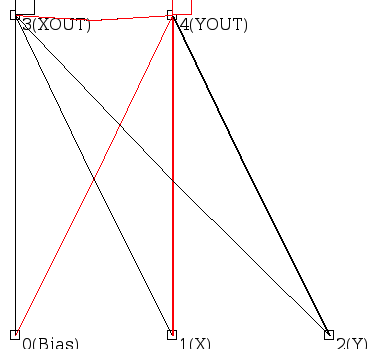
\includegraphics[height=2in]{../../rec/networks/bigeye_13.png}
    } \\
    \subfigure[]{
        \label{fig:bigeye:arnold}
        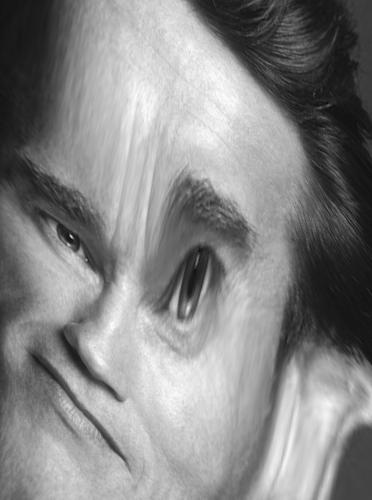
\includegraphics[height=1.8in]{../../rec/faces_distorted/bigeye_13_arnold_schwarzenegger.jpg}
    }
    \subfigure[]{
        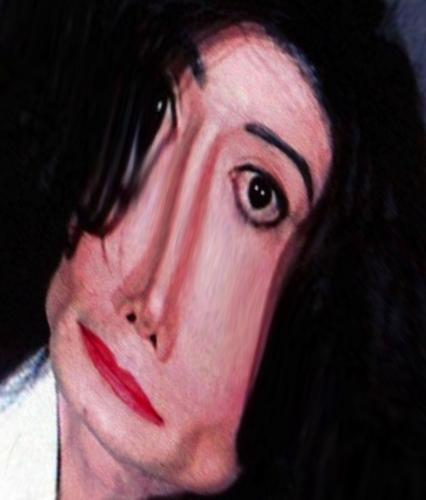
\includegraphics[height=1.8in]{../../rec/faces_distorted/bigeye_13_michael_jackson.jpg}
    } \\
    \subfigure[]{
        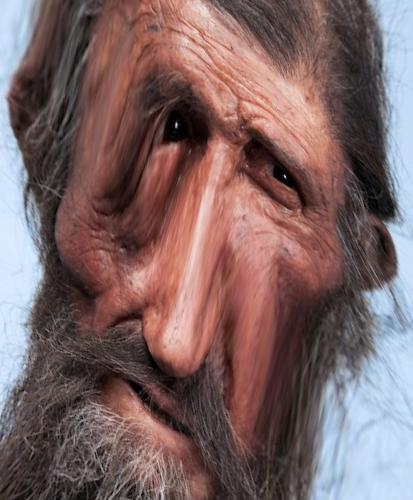
\includegraphics[height=1.8in]{../../rec/faces_distorted/bigeye_13_old_man.jpg}
    }
    \subfigure[]{
        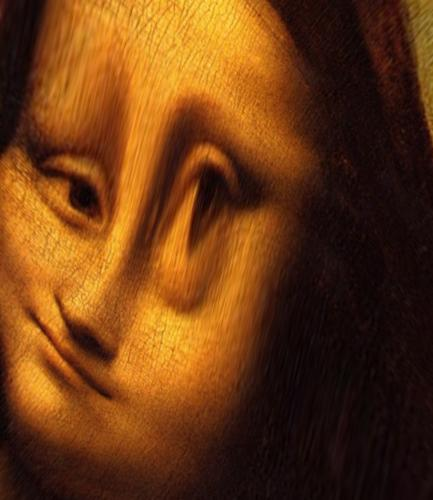
\includegraphics[height=1.8in]{../../rec/faces_distorted/bigeye_13_mona_lisa.jpg}
    } \\
    \subfigure[]{
        \label{fig:bigeye:spongebob}
        
\includegraphics[height=1.8in]{../../rec/faces_distorted/bigeye_13_spongebob.jpg}
    }
    \caption{Big-eye distortion: \ref{fig:bigeye:network} the network and \ref{fig:bigeye:arnold}-\ref{fig:bigeye:spongebob} the distorted face set.\label{fig:bigeye}}
\end{figure*}

\begin{figure*}
    \centering
    \subfigure[]{
        \label{fig:multieye:network}
        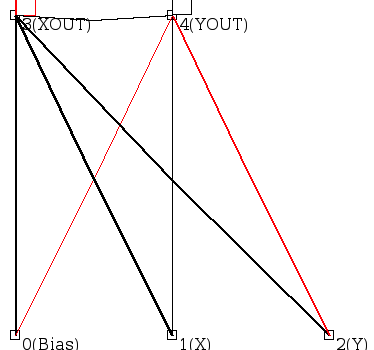
\includegraphics[height=2in]{../../rec/networks/multieye_1.png}
    } \\
    \subfigure[]{
        \label{fig:multieye:arnold}
        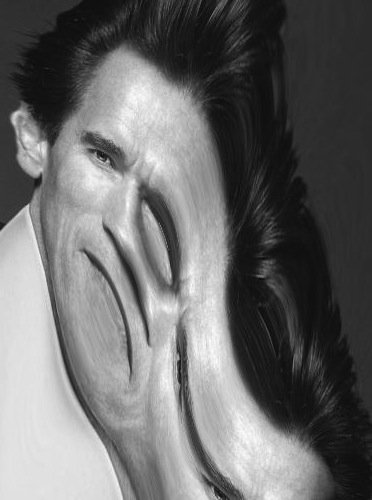
\includegraphics[height=1.8in]{../../rec/faces_distorted/multieye_1_arnold_schwarzenegger.jpg}
    }
    \subfigure[]{
        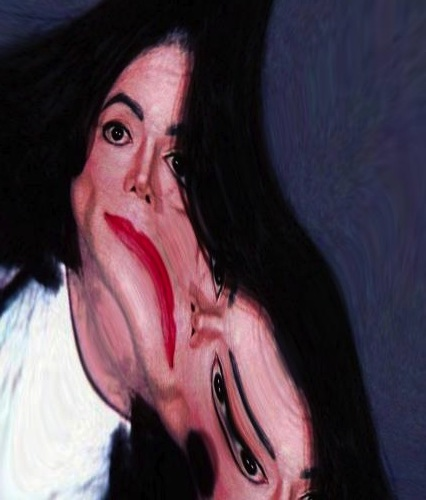
\includegraphics[height=1.8in]{../../rec/faces_distorted/multieye_1_michael_jackson.jpg}
    } \\
    \subfigure[]{
        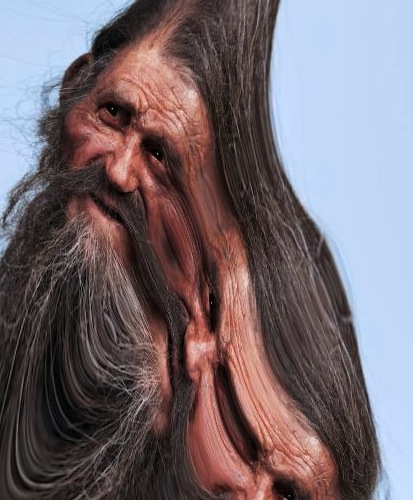
\includegraphics[height=1.8in]{../../rec/faces_distorted/multieye_1_old_man.jpg}
    }
    \subfigure[]{
        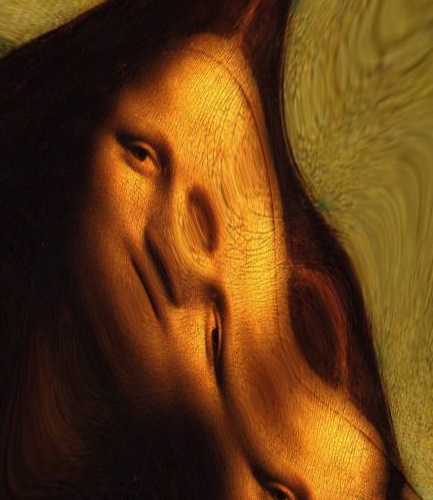
\includegraphics[height=1.8in]{../../rec/faces_distorted/multieye_1_mona_lisa.jpg}
    } \\
    \subfigure[]{
        \label{fig:multieye:spongebob}
        
\includegraphics[height=1.8in]{../../rec/faces_distorted/multieye_1_spongebob.jpg}
    }
    \caption{Multi-eye distortion: \ref{fig:multieye:network} the network and \ref{fig:multieye:arnold}-\ref{fig:multieye:spongebob} the distorted face set.\label{fig:multieye}}
\end{figure*}

\begin{figure*}
    \centering
    \subfigure[]{
        \label{fig:gauss_v:network}
        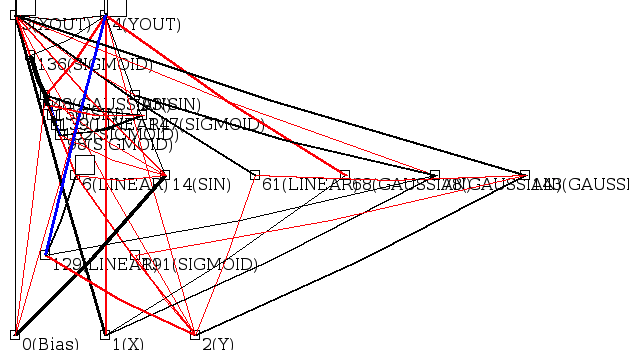
\includegraphics[height=2in]{../../rec/networks/gauss_v_12.png}
    } \\
    \subfigure[]{
        \label{fig:gauss_v:arnold}
        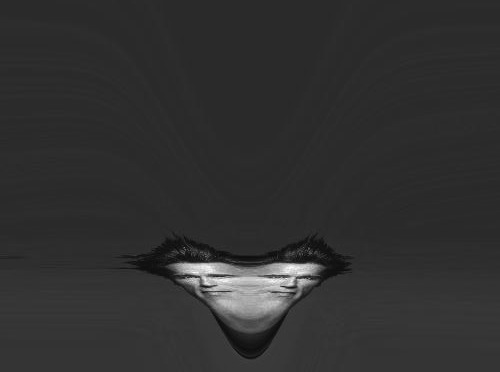
\includegraphics[height=1.8in]{../../rec/faces_distorted/gauss_v_12_arnold_schwarzenegger.jpg}
    }
    \subfigure[]{
        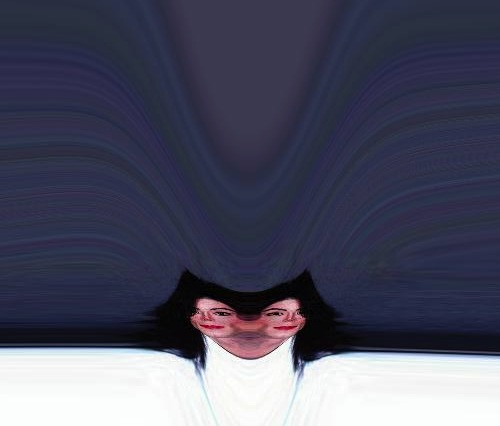
\includegraphics[height=1.8in]{../../rec/faces_distorted/gauss_v_12_michael_jackson.jpg}
    } \\
    \subfigure[]{
        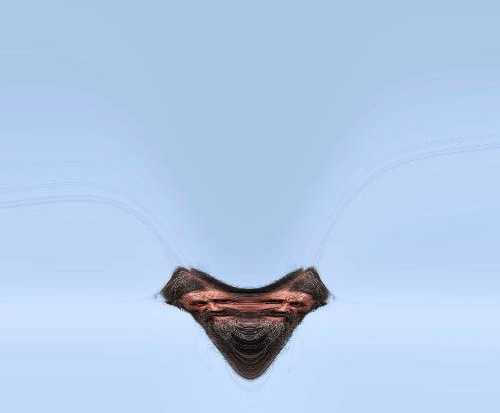
\includegraphics[height=1.8in]{../../rec/faces_distorted/gauss_v_12_old_man.jpg}
    }
    \subfigure[]{
        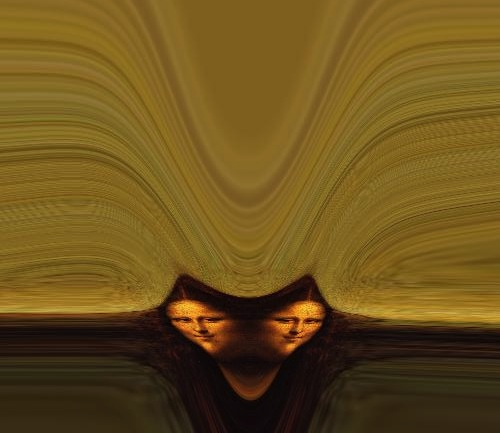
\includegraphics[height=1.8in]{../../rec/faces_distorted/gauss_v_12_mona_lisa.jpg}
    } \\
    \subfigure[]{
        \label{fig:gauss_v:spongebob}
        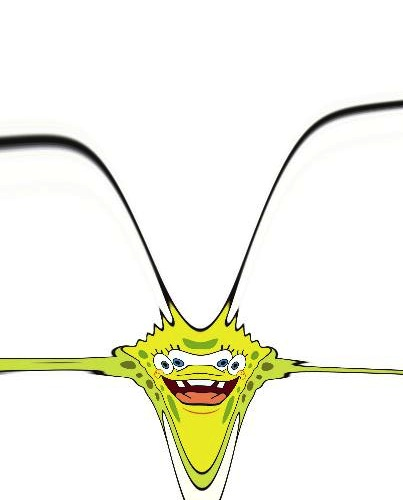
\includegraphics[height=1.8in]{../../rec/faces_distorted/gauss_v_12_spongebob.jpg}
    }
    \caption{Gaussian V distortion: \ref{fig:gauss_v:network} the network and \ref{fig:gauss_v:arnold}-\ref{fig:gauss_v:spongebob} the distorted face set.\label{fig:gauss_v}}
\end{figure*}

\begin{figure*}
    \centering
    \subfigure[]{
        \label{fig:color_extraction:network}
        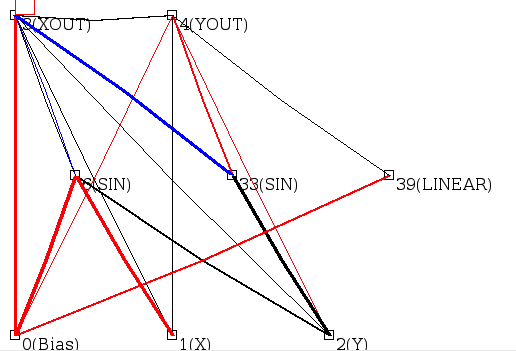
\includegraphics[height=2in]{../../rec/networks/spongebob__colors_extracted__13.png}
    } \\
    \subfigure[]{
        \label{fig:color_extraction:arnold}
        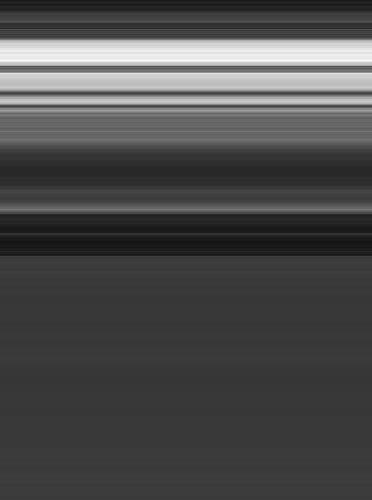
\includegraphics[height=1.8in]{../../rec/faces_distorted/spongebob__colors_extracted__13_arnold_schwarzenegger.jpg}
    }
    \subfigure[]{
        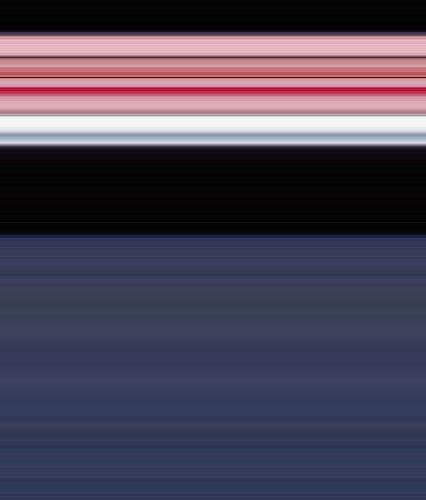
\includegraphics[height=1.8in]{../../rec/faces_distorted/spongebob__colors_extracted__13_michael_jackson.jpg}
    } \\
    \subfigure[]{
        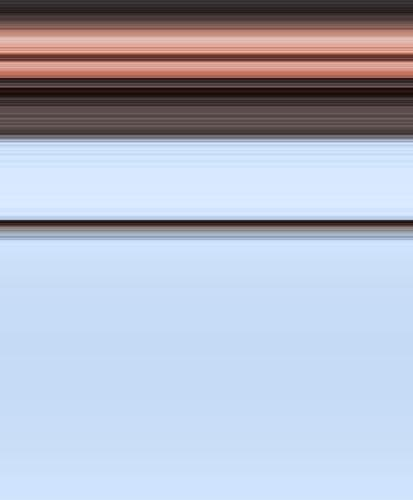
\includegraphics[height=1.8in]{../../rec/faces_distorted/spongebob__colors_extracted__13_old_man.jpg}
    }
    \subfigure[]{
        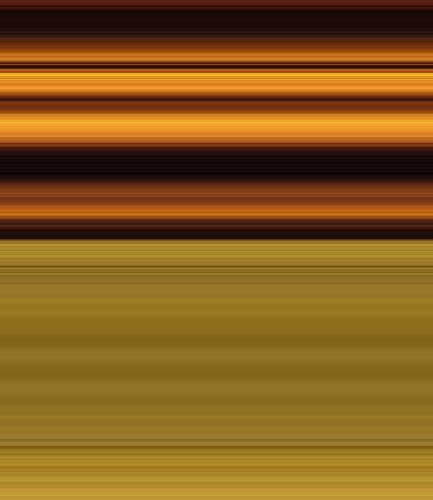
\includegraphics[height=1.8in]{../../rec/faces_distorted/spongebob__colors_extracted__13_mona_lisa.jpg}
    } \\
    \subfigure[]{
        \label{fig:color_extraction:spongebob}
        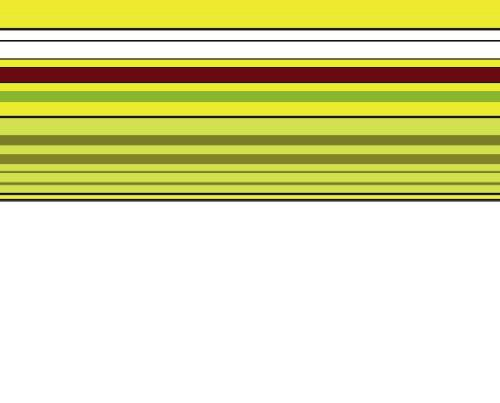
\includegraphics[height=1.8in]{../../rec/faces_distorted/spongebob__colors_extracted__13_spongebob.jpg}
    }
    \caption{Color extraction distortion: \ref{fig:color_extraction:network} the network and \ref{fig:color_extraction:arnold}-\ref{fig:color_extraction:spongebob} the distorted face set.\label{fig:color_extraction}}
\end{figure*}

\section{Discussion}
The experimentation and results yielded some useful findings regarding the work and its usefulness.

First, sending in raw face images alone without any uniformity in or designation of features (such as the head dimensions, eye sizes and locations, et cetera) will not necessarily yield similar results across multiple faces. There were some examples presented showing different eyes elongated for example. Given the networks are configured to flow from the output destination to the source pixel location there is no coherent way to indicate the location of features since those are not known until the deformation is performed. One possibility to look at is reversing the flow of information so that the source locations are input and the destination locations are output. This may cause some issues with sparsely populated image generation which, depending on the distortion, may be difficult or even impossible to fix with blending and interpolation techniques. Another possibly more practical method might be to detect the features in the face image then allow warping to be done on the features individually and recombined to form a face. This has the disadvantage of compartmentalizing individual components though.

Second, interesting results can be obtained with very little complexity but the results tend to converge to similar designs. Even a few hidden nodes can greatly increase the diversity in the results. But to get past this initial no diversity hump the boosting effort seemed fairly useful. Another option might have been to simply start the network off with a few hidden nodes but that approach requires some assumptions in determining what might compose a desirable network, a task that's fairly complicated even with few nodes. For example, is figure \ref{fig:color_extraction} desirable? One may suppose it depends largely on the application; for general face deformations it's probably not very interesting. It's difficult to deduce beforehand that two sine nodes and one linear won't make something interesting and it's difficult to deduce that they won't ever create something interesting. The other aspect of boosting that is of interest is the part played by the cross correlation. It seemed to perform well at discriminating close to duplicates but they had to be very close for it to be useful. This may very well not be the best similarity indication available. Even if it were there would need to be large speed improvements made before it could be considered practical. This may very well come out of simply moving it away from Python into C or C++.

Third, the technique as it is currently implemented may have limited practical use on real images or detailed drawings but it seems to have some clear applications in less detailed use cases. The cartoons generated, for instance, show some potential of the system to evolve cartoons and, if expanded into a three dimensional space, perhaps also structures. This could be an interesting addition if trying to generate unique user-generated data (in games, for example).

\section{Future Work}
The experiments presented in this report have yielded a fairly diverse and interesting set of outcomes but by no means is it argued that the results and the experimental method is optimal, assuming there is an optimum to be found. From this point there are many avenues of research that might yield more varied, structured, and interesting results. Here some ideas for future progress will be presented.

Given the technology as it stands it would be interesting to see more results of a more widespread use of the application. Due to the inherent biases in the operators conducting the research, some artificial limits due to operator likes and dislikes could certainly be constraining the discovery of many interesting distortions. A PicBreeder style community approach might be interesting to see.

Two methods were developed as a result of this research to boost the generation of complexity in the networks: the more conservative cross correlation approach and the bit more extreme uncorrelated random burst approach. The random burst approach is not necessarily well suited for building desirable complexity as opposed to simply random complexity, but it is very fast. The cross correlation does a somewhat better job, but it can only detect pixel by pixel image similarities, and only among the set the cross correlation is run against. Because of the time required to run the algorithm the only images correlated were among a single generation. This removes the possibility of ignoring similar images found in past generations. These two limitations, that of speed and that of limited history, can perhaps be mitigated by uncovering better approaches to the calculations or the method used entirely. Developing filtering and complexification methodologies that are not quite so time consuming might make the process more useful and friendly to an operator with limited time.

As mentioned previously, though some ideas were explored this research was unable to uncover an effective method for creating pose and proportion invariant distortions. It is believed that for the distortions to have any sort of practical application they should be less dependent on the unique spatial properties and orientations of the images they're evolved with. It would certainly be interesting to see this hurdle overcome.

This research has unveiled some interesting possibilities of the technique when used on cartoon images. As mentioned previously this technique could be useful in artificial user-created worlds. It is feasible to see how an algorithm might be able to convert the deformed cartoon image into a more structured creature. It would be interesting to see this avenue explored further.

This has been a fairly limited selection of the possibilities for expansion and it is easy to see this technology is quite open ended in method and application so the potential for future work is necessarily unbounded as far as one can see.

\section{Conclusion}
The goal of the research conducted and presented in this report was to explore the realm of possibilities around interactive evolution of CPPN neural networks as applied to the domain of warping bitmap images of human faces and, to some extent, anthropomorphic variations. The research was able to demonstrate a useful application allowing a user to interactively evolve the distortion on an image input to the system. The research conducted was also able to unveil some useful approaches toward boosting the effectiveness of the interactive evolutionary process through the previously mentioned correlated and uncorrelated approaches while also discussing their respective advantages and disadvantages. Presented here are some of the results obtained and some analysis of them and their origination. This research has also helped to identify some new avenues for research as well as illuminate some possible applications of the technology.

\bibliographystyle{IEEEtran}
\bibliography{references.bib}

\end{document}